\chapter{Kurva Arus--Potensial}\label{ch:b2:current-potential-curves}

Seng dilapiskan secara elektrolitik pada baja dari bak-bak asam. Padahal
diagram E--pH dari jilid Tahun 1 menyatakan bahwa seng, yang jauh di bawah
garis hidrogen, seharusnya mereduksi asam dan larut secepat seng itu
diendapkan. Hal itu tidak terjadi, karena sebuah diagram menyatakan apa
yang mungkin terjadi, bukan seberapa cepat. Laju reaksi elektrode adalah
sebuah arus, dan mengalurkan arus itu terhadap potensial elektrode
langsung memperlihatkan reaksi mana yang cepat, mana yang lambat, dan mana
yang tertahan oleh pasokan pereaksi. \omterm{def:b2:current-potential-curves:ie-curve}{Kurva arus--potensial} ini adalah alat
setiap ahli elektrokimia yang melapisi logam, mengisi baterai, atau
mengukur oksigen di sungai.

\begin{recall}
Jilid Tahun 1: potensial elektrode, elektrode acuan, persamaan Nernst,
diagram E--pH dan batasnya (diagram itu menyatakan apa yang mungkin, bukan
seberapa cepat). \Cref{ch:b2:cell-thermodynamics}: $\Delta_r G = -nFE$,
persamaan Nernst yang diturunkan. Dari fisika: difusi dan hukum Fick,
$j = -D\,dc/dx$.
\end{recall}

\begin{omfigure}
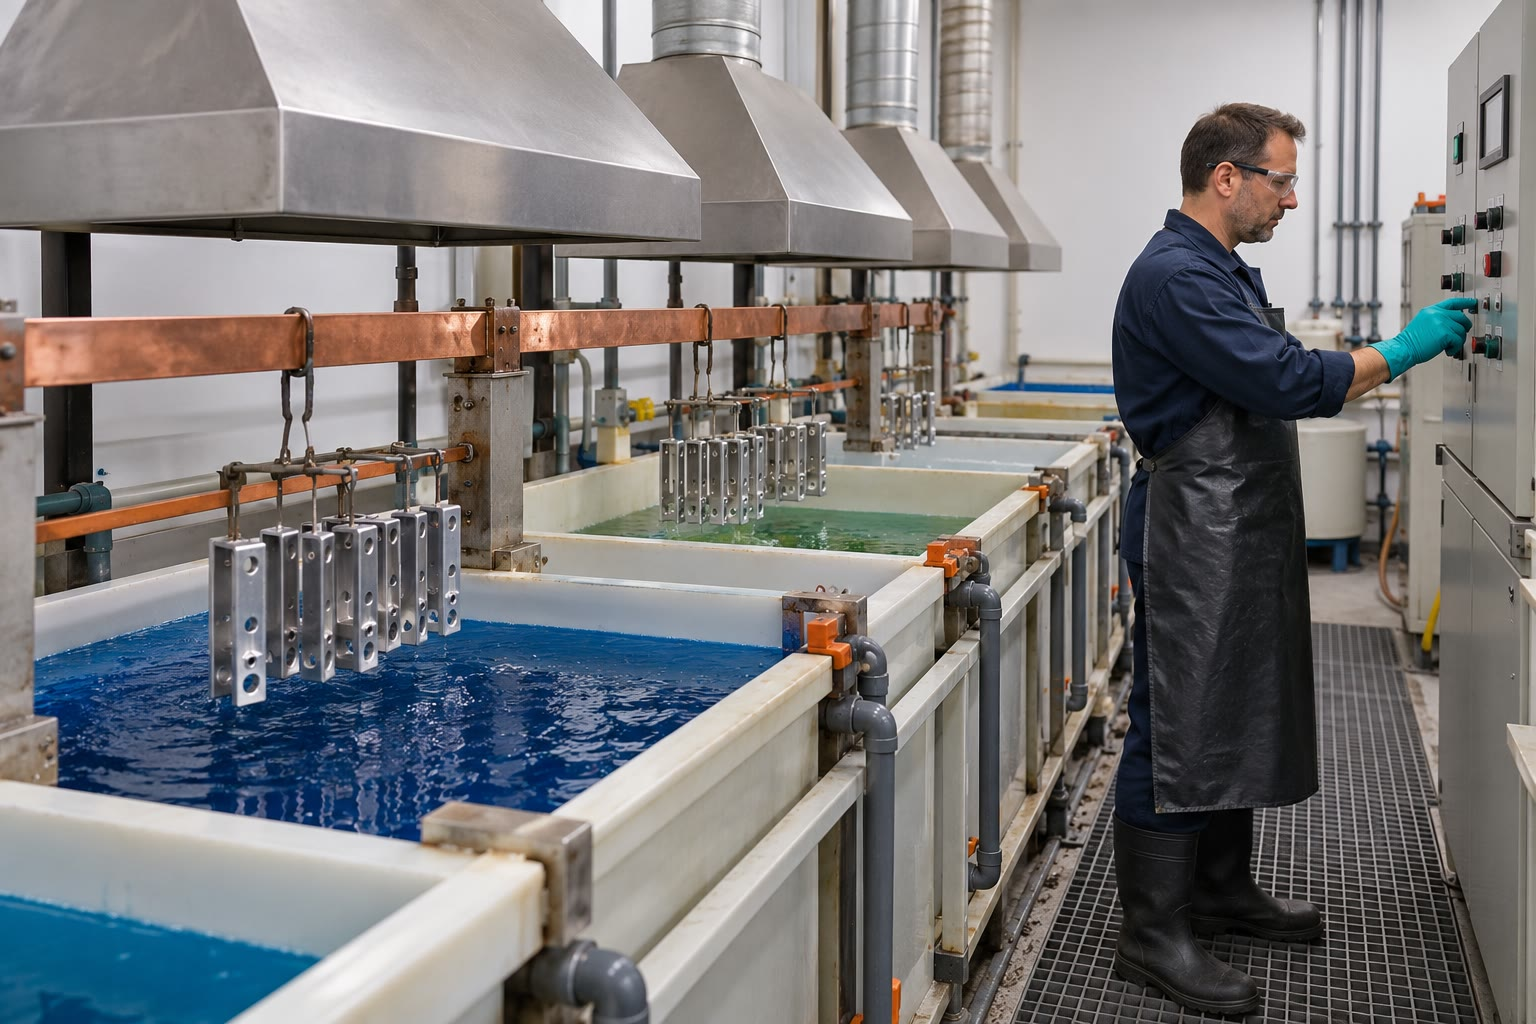
\includegraphics[width=0.62\linewidth]{images/book3/ai/b2-10-electroplating.jpg}

{\small Jalur pelapisan listrik: benda-benda yang akan dilapisi digantung
pada batang-batang tembaga ke dalam bak dan dijadikan katode; operator
mengatur arus pada penyearah. Arus menetapkan seberapa cepat logam
diendapkan; potensial benda-benda itu menentukan logam mana, atau berapa
banyak hidrogen, yang terbentuk bersamanya.}
\end{omfigure}

\section{Elektrode di luar kesetimbangan}

\begin{definition}[Kurva arus--potensial]\label{def:b2:current-potential-curves:ie-curve}
Yang disebut \emph{kurva arus--potensial}\index{kurva arus--potensial}
sebuah elektrode dalam suatu larutan adalah grafik arus $i$ yang melewati
elektrode itu terhadap potensialnya $E$. Sebuah \emph{arus
anodik}\index{arus anodik}, yang dihitung positif, bersesuaian dengan
oksidasi pada elektrode; sebuah \emph{arus katodik}\index{arus katodik},
yang dihitung negatif, dengan reduksi.
\end{definition}

\begin{definition}[Spesies elektroaktif]\label{def:b2:current-potential-curves:electroactive}
Yang disebut \emph{spesies elektroaktif}\index{spesies elektroaktif}
adalah spesies yang dapat dioksidasi atau direduksi pada elektrode dalam
rentang potensial yang ditinjau.
\end{definition}

\begin{proposition}[Arus dan laju]\label{prop:b2:current-potential-curves:current-rate}
Jika satu setengah reaksi dengan $n$ elektron berlangsung pada sebuah
elektrode, arus mengukur lajunya: $i = nF\,d\xi/dt$, dengan $\xi$ kemajuan
oksidasi (sehingga $i > 0$ untuk oksidasi, $i < 0$ untuk reduksi).
\end{proposition}

\begin{proof}
Menurut \cref{prop:b2:cell-thermodynamics:charge}, kemajuan $d\xi$
memindahkan muatan $nF\,d\xi$ melalui elektrode dalam waktu $dt$.
\end{proof}

Untuk merekam kurva semacam itu, potensial sebuah elektrode harus
ditetapkan dan diukur sementara arus mengalir melaluinya --- yang tidak
dapat dilakukan oleh sel dua elektrode, karena arus juga mengubah potensial
elektrode kedua.

\begin{definition}[Susunan tiga elektrode]\label{def:b2:current-potential-curves:set-up}
Dalam susunan tiga elektrode, arus mengalir antara \emph{elektrode
kerja}\index{elektrode kerja}, yaitu elektrode yang dipelajari, dan \emph{elektrode lawan}\index{elektrode lawan},
yang menutup rangkaian; potensial elektrode kerja diukur terhadap
elektrode acuan yang tidak dilewati arus. Sebuah potensiostat elektronik
mengatur arus sedemikian rupa sehingga potensial itu tetap pada nilai yang
ditetapkan.
\end{definition}

\begin{omfigure}
\begin{tikzpicture}[font=\small, >={Stealth}]
  \pic[transform shape] at (0,0) {beaker={0.7}{omDef!14}};
  \pic at (-0.55,0.25) {electrode={black!35}};
  \pic at (0.55,0.25) {electrode={black!15}};
  \pic (r) at (0.0,0.15) {probe};
  \draw[thick, rounded corners] (-2.2,4.3) rectangle (2.2,5.5);
  \node at (0,4.9) {potensiostat};
  \draw[thick, omThm] (-0.40,2.65) -- (-0.40,3.5) -- (-1.6,3.5) -- (-1.6,4.3);
  \draw[thick, omDef] (0.70,2.65) -- (0.70,3.5) -- (1.6,3.5) -- (1.6,4.3);
  \draw[thick] (r-top) -- (0,4.3);
  \node[anchor=east, font=\scriptsize, omThm] at (-1.65,3.85) {EK};
  \node[anchor=west, font=\scriptsize, omDef] at (1.65,3.85) {EL};
  \node[anchor=west, font=\scriptsize] at (0.05,3.95) {EA};
  \draw[<-, omProp, thick] (-0.75,1.2) -- (-2.0,1.4) node[left, text=black, align=right] {elektrode\\ kerja};
  \draw[<-, omProp, thick] (0.85,1.2) -- (2.1,1.4) node[right, text=black, align=left] {elektrode\\ lawan};
  \draw[<-, omProp, thick] (0.05,0.5) -- (1.4,-0.4) node[right, text=black] {elektrode acuan};
  \node[font=\scriptsize, align=center] at (0,6.0) {menetapkan $E_{\text{EK}} - E_{\text{EA}}$, mengukur $i$};
\end{tikzpicture}

{\small Susunan tiga elektrode. Potensiostat mengalirkan arus antara
\omterm{def:b2:current-potential-curves:set-up}{elektrode kerja} (EK) dan \omterm{def:b2:current-potential-curves:set-up}{elektrode lawan} (EL) untuk mempertahankan
potensial \omterm{def:b2:current-potential-curves:set-up}{elektrode kerja}, yang diukur terhadap elektrode acuan (EA),
pada nilai yang ditetapkan; tidak ada arus yang melewati elektrode
acuan.}
\end{omfigure}

Jika tidak ada arus yang mengalir dan kedua bentuk sebuah pasangan ada,
elektrode mengambil potensial Nernst pasangan itu --- jika pertukaran
elektronnya cukup cepat untuk menegakkannya. Menggeser potensial menjauh
dari nilai itu membuat arus mengalir.

\section{Sistem cepat dan sistem lambat}

\begin{definition}[Overpotensial]\label{def:b2:current-potential-curves:overpotential}
Yang disebut \emph{overpotensial}\index{overpotensial} sebuah elektrode
yang dilewati arus $i$ adalah $\eta = E(i) - E_{\text{eq}}$, yaitu selisih
antara potensialnya dan potensial kesetimbangan (Nernst) pasangan itu.
Yang disebut \emph{potensial ambang}\index{potensial ambang} sebuah
setengah reaksi adalah potensial yang setelah dilampaui membuat arusnya
menjadi berarti.
\end{definition}

\begin{definition}[Sistem cepat dan sistem lambat]\label{def:b2:current-potential-curves:fast-slow}
Sebuah pasangan disebut \emph{sistem cepat}\index{sistem cepat} pada
elektrode tertentu jika arus yang berarti langsung mengalir begitu
potensialnya menjauh dari potensial Nernst-nya; pasangan itu disebut
\emph{sistem lambat}\index{sistem lambat} jika diperlukan \omterm{def:b2:current-potential-curves:overpotential}{overpotensial}
sebesar beberapa persepuluh volt sebelum arusnya menjadi berarti, ke arah
mana pun.
\end{definition}

Cepat atau lambatnya sebuah sistem bergantung pada pasangan dan pada bahan
elektrode. Pasangan \ce{Fe^3+}/\ce{Fe^2+} dan \ce{Ag+}/\ce{Ag} cepat pada
platina; reduksi \ce{H+} cepat pada platina tetapi lambat pada raksa,
timbal, atau seng; oksidasi air menjadi dioksigen lambat pada setiap
elektrode. Transfer elektron yang memutus atau membentuk ikatan, seperti
pada \ce{O2} atau \ce{H2}, biasanya lambat; transfer satu elektron di
antara dua ion yang bentuknya hampir sama berlangsung cepat. Bentuk bagian
kurva lambat yang menanjak berasal dari kinetika transfer elektron, yang
diturunkan dalam jilid Tahun 3.

\begin{omfigure}
\begin{tikzpicture}
\begin{axis}[omie, width=0.47\linewidth, height=5.4cm, xmin=0.25, xmax=1.3,
  ymin=-1.3, ymax=1.3, xlabel={$E$}, ylabel={$i$}, title={\small sistem cepat}]
\addplot[omanodic] table[x=E, y=i, restrict expr to domain={\thisrow{i}}{0:2}] {figdata/out/bachelor-2-ie-curves-a.dat};
\addplot[omcathodic] table[x=E, y=i, restrict expr to domain={\thisrow{i}}{-2:0}] {figdata/out/bachelor-2-ie-curves-a.dat};
\draw[densely dotted] (axis cs:0.77,-1.2) -- (axis cs:0.77,1.2);
\node[font=\scriptsize, anchor=north west] at (axis cs:0.78,-0.05) {$E_{\text{eq}}$};
\node[font=\scriptsize, anchor=south] at (axis cs:1.1,1.0) {\ce{Fe^2+} $\to$ \ce{Fe^3+}};
\node[font=\scriptsize, anchor=north] at (axis cs:0.45,-1.0) {\ce{Fe^3+} $\to$ \ce{Fe^2+}};
\end{axis}
\end{tikzpicture}\hfill
\begin{tikzpicture}
\begin{axis}[omie, width=0.47\linewidth, height=5.4cm, xmin=-0.25, xmax=1.8,
  ymin=-1.3, ymax=1.3, xlabel={$E$}, ylabel={$i$}, title={\small sistem lambat}]
\addplot[omanodic] table[x=E, y=i, restrict expr to domain={\thisrow{i}}{0:2}] {figdata/out/bachelor-2-ie-curves-c.dat};
\addplot[omcathodic] table[x=E, y=i, restrict expr to domain={\thisrow{i}}{-2:0}] {figdata/out/bachelor-2-ie-curves-c.dat};
\draw[densely dotted] (axis cs:0.77,-1.2) -- (axis cs:0.77,1.2);
\draw[<->, omProp] (axis cs:0.77,0.5) -- (axis cs:1.12,0.5) node[midway, above, font=\scriptsize] {$\eta_a$};
\draw[<->, omProp] (axis cs:0.42,-0.5) -- (axis cs:0.77,-0.5) node[midway, below, font=\scriptsize] {$\eta_c$};
\node[font=\scriptsize, anchor=north west] at (axis cs:0.78,-0.05) {$E_{\text{eq}}$};
\end{axis}
\end{tikzpicture}

{\small \omterm{def:b2:current-potential-curves:ie-curve}{Kurva arus--potensial} model sebuah pasangan yang kedua bentuknya ada
dengan konsentrasi yang sama (cabang anodik merah, katodik biru). Kiri,
\omterm{def:b2:current-potential-curves:fast-slow}{sistem cepat}: arus berganti tanda secara tajam pada potensial
kesetimbangan. Kanan, \omterm{def:b2:current-potential-curves:fast-slow}{sistem lambat}: tidak ada arus yang mengalir dalam
suatu rentang potensial di sekitarnya; setiap cabang memerlukan
\omterm{def:b2:current-potential-curves:overpotential}{overpotensial}. Keduanya mencapai plato pembatas yang sama, yang
ditetapkan oleh difusi. (Nilai-nilai ilustratif.)}
\end{omfigure}

\section{Transpor massa dan arus pembatas}

Jika transfer elektronnya cepat, arus dibatasi oleh kedatangan pereaksi di
elektrode. Dalam larutan yang diaduk, lapisan tipis cairan di dekat
elektrode tetap hampir diam, dan pereaksi melintasinya dengan difusi.

\begin{definition}[Lapisan difusi dan arus pembatas]\label{def:b2:current-potential-curves:limiting-current}
Yang disebut \emph{lapisan difusi}\index{lapisan difusi} adalah lapisan
larutan setebal $\delta$ (beberapa sampai beberapa puluh mikrometer dalam
larutan yang diaduk) di dekat elektrode, yang dilintasi spesies hanya
dengan difusi. Yang disebut \emph{arus pembatas}\index{arus pembatas}
adalah arus yang dicapai ketika \omterm{def:b2:current-potential-curves:electroactive}{spesies elektroaktif} dikonsumsi secepat
kedatangannya, sehingga konsentrasinya di permukaan sama dengan nol.
\end{definition}

\begin{omfigure}
\begin{tikzpicture}[font=\small, >={Stealth}, x=1.2cm, y=1.2cm]
  \fill[black!25] (-0.4,0) rectangle (0,3);
  \node[rotate=90, font=\scriptsize] at (-0.2,1.5) {elektrode};
  \draw[->] (0,0) -- (4.6,0) node[right] {$x$};
  \draw[->] (0,0) -- (0,3.2) node[above] {$c$};
  \draw[densely dashed] (1.6,0) -- (1.6,3);
  \node[below, font=\scriptsize] at (1.6,0) {$\delta$};
  \draw[omDef, thick] (0,1.2) -- (1.6,2.4) -- (4.4,2.4);
  \draw[omThm, thick] (0,0.02) -- (1.6,2.4);
  \node[font=\scriptsize, anchor=west] at (2.6,2.6) {ruah, $c^b$ (diaduk)};
  \node[font=\scriptsize, omDef, anchor=east] at (-0.45,1.2) {$c^s$};
  \node[font=\scriptsize, omThm, anchor=west] at (1.7,0.5) {$c^s = 0$: arus pembatas};
  \node[font=\scriptsize, align=center] at (0.8,3.0) {lapisan\\ difusi};
\end{tikzpicture}

{\small Konsentrasi pereaksi di dekat elektrode dalam larutan yang diaduk.
Di sepanjang \omterm{def:b2:current-potential-curves:limiting-current}{lapisan difusi} profilnya linear; fluks, dan dengan demikian
arus, sebanding dengan $c^b - c^s$. Fluks itu paling besar ketika pereaksi
dikonsumsi begitu tiba ($c^s = 0$, merah).}
\end{omfigure}

\begin{theorem}[Arus pembatas]\label{thm:b2:current-potential-curves:limiting}
Untuk spesies dengan konsentrasi ruah $c$ dan koefisien difusi $D$, yang
melintasi \omterm{def:b2:current-potential-curves:limiting-current}{lapisan difusi} setebal $\delta$ menuju elektrode seluas $A$, \omterm{def:b2:current-potential-curves:limiting-current}{arus
pembatasnya}, dalam nilai mutlak, adalah
\[
  |i_{\lim}| = \frac{nFADc}{\delta} .
\]
\end{theorem}

\begin{proof}
Dalam keadaan tunak, profil konsentrasi di dalam lapisan itu linear (hukum
kedua Fick dengan $\partial c/\partial t = 0$ memberikan $d^2c/dx^2 = 0$),
sehingga fluks menuju elektrode adalah $j = D(c - c^s)/\delta$, dalam mol
per satuan luas per satuan waktu. Setiap molekul yang tiba bereaksi dengan
$n$ elektron: $|i| = nFAj =
nFAD(c - c^s)/\delta$, paling besar untuk
$c^s = 0$.
\end{proof}

\begin{example}[Besarnya arus pembatas]\label{ex:b2:current-potential-curves:ilim}
Untuk spesies dengan konsentrasi \qty{10}{mmol/L} (\qty{10}{mol/m^3}),
dengan $D =
\qty{7e-10}{m^2/s}$, $\delta = \qty{20}{\micro m}$, $n = 1$,
pada \qty{1.0}{cm^2}: $|i_{\lim}| = 96\,485 \times 10^{-4} \times 7 \times 10^{-10}
\times 10/(2 \times 10^{-5}) = \qty{3.4}{mA}$.
\end{example}

\begin{theorem}[Gelombang sistem cepat]\label{thm:b2:current-potential-curves:wave}
Untuk pasangan cepat $\mathrm{Ox} + n\,\mathrm e^- \rightleftharpoons \mathrm{Red}$,
dengan \omterm{def:b2:current-potential-curves:limiting-current}{arus pembatas} anodik $i_{\lim,a} > 0$ (yang ditetapkan oleh Red) dan
\omterm{def:b2:current-potential-curves:limiting-current}{arus pembatas} katodik $i_{\lim,c} < 0$ (yang ditetapkan oleh Ox), kurva
keadaan tunaknya adalah
\[
  E = E_{1/2} + \frac{RT}{nF}\ln\frac{i - i_{\lim,c}}{i_{\lim,a} - i},
  \qquad E_{1/2} = E^\circ + \frac{RT}{nF}\ln\frac{D_{\text{Red}}}{D_{\text{Ox}}} ,
\]
dengan tebal lapisan yang sama untuk kedua bentuk.
\end{theorem}

\begin{proof}
\omterm{def:b2:current-potential-curves:fast-slow}{Sistem cepat}: persamaan Nernst berlaku di permukaan,
$E = E^\circ + (RT/nF)
\ln(c^s_{\text{Ox}}/c^s_{\text{Red}})$. Profil linear:
\omterm{def:b2:current-potential-curves:ie-curve}{arus anodik} $i$ mengonsumsi bentuk tereduksi dan menghasilkan bentuk
teroksidasi di permukaan,
$i = nFAD_{\text{Red}}(c^b_{\text{Red}}
- c^s_{\text{Red}})/\delta = -nFAD_{\text{Ox}}(c^b_{\text{Ox}} - c^s_{\text{Ox}})/\delta$.
Dengan $i_{\lim,a} = nFAD_{\text{Red}}c^b_{\text{Red}}/\delta$ dan
$i_{\lim,c} =
-nFAD_{\text{Ox}}c^b_{\text{Ox}}/\delta$, hubungan-hubungan
ini memberikan $c^s_{\text{Red}} = (i_{\lim,a} -
i)\delta/(nFAD_{\text{Red}})$ dan
$c^s_{\text{Ox}} = (i - i_{\lim,c})\delta/(nFAD_{\text{Ox}})$.
Substitusikan ke dalam persamaan Nernst.
\end{proof}

\begin{corollary}[Potensial setengah gelombang]\label{cor:b2:current-potential-curves:half-wave}
Jika kedua bentuk mempunyai koefisien difusi yang sama, $E_{1/2} = E^\circ$:
dengan hanya satu bentuk yang ada, arus bernilai setengah nilai
pembatasnya pada potensial standar pasangan itu.
\end{corollary}

\begin{proof}
Dengan hanya bentuk tereduksi yang ada, $i_{\lim,c} = 0$, dan untuk $i = i_{\lim,a}/2$
logaritmanya nol: $E = E_{1/2} = E^\circ$ jika $D_{\text{Red}} = D_{\text{Ox}}$.
\end{proof}

\begin{proposition}[Plato mengukur konsentrasi]\label{prop:b2:current-potential-curves:plateau}
Dengan pengadukan dan elektrode yang tetap, tinggi sebuah plato sebanding
dengan konsentrasi spesies yang dikonsumsinya: elektrode yang dijaga pada
potensial di atas plato merupakan sensor amperometrik.
\end{proposition}

\begin{proof}
$|i_{\lim}| = (nFAD/\delta)\,c$, dan faktor dalam tanda kurung tetap pada
pengadukan dan suhu yang tetap.
\end{proof}

\begin{omfigure}
\begin{tikzpicture}
\begin{axis}[omie, width=0.47\linewidth, height=5.0cm, xmin=0.25, xmax=1.3,
  ymin=-0.3, ymax=1.3, xlabel={$E$}, ylabel={$i$}, title={\small hanya ada \ce{Fe^2+}}]
\addplot[omanodic] table[x=E, y=i] {figdata/out/bachelor-2-ie-curves-b.dat};
\draw[densely dotted] (axis cs:0.77,0) -- (axis cs:0.77,0.5) -- (axis cs:0.25,0.5);
\node[font=\scriptsize, anchor=north] at (axis cs:0.77,-0.02) {$E_{1/2}$};
\node[font=\scriptsize, anchor=south west] at (axis cs:0.27,0.5) {$i_{\lim}/2$};
\node[font=\scriptsize, anchor=south] at (axis cs:1.12,1.0) {plato};
\end{axis}
\end{tikzpicture}\hfill
\begin{tikzpicture}
\begin{axis}[width=0.42\linewidth, height=5.0cm, xmin=0, xmax=1.05, ymin=0, ymax=1.1,
  axis x line=bottom, axis y line=left, xtick=\empty, ytick=\empty,
  xlabel={$c$}, ylabel={$i_{\lim}$}, label style={font=\small},
  title={\small amperometri}]
\addplot[omanodic, mark=*, mark size=1.2pt] table[x=c, y=i] {figdata/out/bachelor-2-ie-curves-e.dat};
\end{axis}
\end{tikzpicture}

{\small Kiri: gelombang pasangan cepat jika hanya bentuk tereduksi yang ada
(model); setengah tingginya terletak pada potensial setengah gelombang.
Kanan: tinggi plato bertambah sebanding dengan konsentrasi.}
\end{omfigure}

\section{Pelarut dan elektrode}

Air sendiri bersifat elektroaktif: air dioksidasi menjadi dioksigen
(\ce{2H2O -> O2 + 4H+ + 4e-}) dan direduksi menjadi dihidrogen
(\ce{2H+ + 2e- -> H2}, atau \ce{2H2O + 2e- -> H2 + 2OH-}). Karena pelarut
tidak pernah habis, kurva-kurvanya tidak mempunyai plato: kurva itu
menanjak tajam dan membatasi setiap kurva lain.

\begin{definition}[Jendela elektroaktivitas]\label{def:b2:current-potential-curves:window}
Yang disebut \emph{dinding pelarut}\index{dinding pelarut} adalah
cabang-cabang curam oksidasi dan reduksi pelarut. Yang disebut
\emph{jendela elektroaktivitas}\index{jendela elektroaktivitas} adalah
rentang potensial di antara keduanya, tempat kurva spesies-spesies
terlarut dapat diamati.
\end{definition}

\begin{proposition}[Jendela air]\label{prop:b2:current-potential-curves:window}
Dalam air pada pH tertentu, jendela itu terletak di sekitar rentang
termodinamika kedua pasangan air, $\qty{0}{V} - 0.059\,\mathrm{pH}$ dan
$\qty{1.23}{V} -
0.059\,\mathrm{pH}$, yang diperlebar di setiap sisi oleh
\omterm{def:b2:current-potential-curves:overpotential}{overpotensial} reaksi yang bersesuaian pada elektrode yang dipakai.
\end{proposition}

\begin{proof}[Argumen]
Setiap dinding dimulai di dekat potensial Nernst pasangannya, yang
digeser oleh \omterm{def:b2:current-potential-curves:overpotential}{overpotensial} ambang: oksidasi air lambat pada semua
elektrode, sehingga dinding anodik terletak beberapa persepuluh volt di
atas \qty{1.23}{V} (pada pH 0); reduksi \ce{H+} cepat pada platina, yang
dinding katodiknya tetap dekat \qty{0}{V}, tetapi lambat pada seng,
timbal, atau raksa, yang dindingnya terletak beberapa persepuluh volt
lebih rendah.
\end{proof}

\begin{omfigure}
\begin{tikzpicture}
\begin{axis}[omie, width=0.82\linewidth, height=5.4cm, xmin=-1.2, xmax=2.0,
  ymin=-3, ymax=3, xlabel={$E$ (V)}, ylabel={$i$}, clip=true, clip mode=individual]
\addplot[omwall] table[x=E, y=i] {figdata/out/bachelor-2-ie-curves-d-high.dat};
\addplot[omcathodic] table[x=E, y=i, restrict expr to domain={\thisrow{E}}{-1.2:0.6}] {figdata/out/bachelor-2-ie-curves-d-Pt.dat};
\addplot[omanodic] table[x=E, y=i, restrict expr to domain={\thisrow{E}}{0.6:2.0}] {figdata/out/bachelor-2-ie-curves-d-Pt.dat};
\draw[densely dotted] (axis cs:0,-2.8) -- (axis cs:0,2.8);
\draw[densely dotted] (axis cs:1.23,-2.8) -- (axis cs:1.23,2.8);
\node[font=\scriptsize, anchor=north west] at (axis cs:0.02,-0.1) {0};
\node[font=\scriptsize, anchor=north west] at (axis cs:1.24,-0.1) {1.23};
\node[font=\scriptsize, omDef, anchor=west] at (axis cs:0.05,-2.2) {\ce{H+} $\to$ \ce{H2} pada Pt};
\node[font=\scriptsize, gray, anchor=east] at (axis cs:-0.85,-1.0) {pada Zn, Pb};
\node[font=\scriptsize, omThm, anchor=east] at (axis cs:1.18,2.2) {\ce{H2O} $\to$ \ce{O2}};
\end{axis}
\end{tikzpicture}

{\small Dinding-dinding air pada pH 0 (model). Reduksi \ce{H+} dimulai di
dekat \qty{0}{V} pada platina (biru) tetapi beberapa persepuluh volt lebih
rendah pada logam seperti seng atau timbal (putus-putus); oksidasi air
memerlukan \omterm{def:b2:current-potential-curves:overpotential}{overpotensial} pada elektrode apa pun. Jendelanya adalah rentang
di antara dinding-dinding itu.}
\end{omfigure}

\section{Membaca kurva}

\begin{method}[Membuat sketsa kurva-kurva sebuah larutan]\label{met:b2:current-potential-curves:sketch-ie}
\begin{enumerate}
  \item Gambarlah kedua \omterm{def:b2:current-potential-curves:window}{dinding pelarut} untuk pH dan bahan elektrode itu.
  \item Untuk setiap pasangan yang ada, letakkan potensial Nernst-nya
        (kedua bentuk ada) atau $E^\circ$ (satu bentuk): \omterm{def:b2:current-potential-curves:fast-slow}{sistem cepat}
        memotong sumbu di sana secara tajam; \omterm{def:b2:current-potential-curves:fast-slow}{sistem lambat} tergeser oleh
        \omterm{def:b2:current-potential-curves:overpotential}{overpotensialnya}.
  \item Berilah setiap gelombang plato yang sebanding dengan konsentrasi
        spesies yang dikonsumsinya; elektrode logam yang mengoksidasi
        dirinya sendiri tidak mempunyai plato (logamnya tidak habis).
  \item Jumlahkan arus reaksi-reaksi yang mungkin pada setiap potensial.
\end{enumerate}
\end{method}

\begin{method}[Membaca kurva-kurva]\label{met:b2:current-potential-curves:read-ie}
\begin{enumerate}
  \item Pada potensial yang ditetapkan, bacalah pada setiap kurva arus
        setiap reaksi: reaksi-reaksi itu berlangsung bersamaan, sebanding
        dengan arusnya.
  \item Pada arus yang ditetapkan (elektrolisis), carilah potensial tempat
        kurva-kurva anodik atau katodik berjumlah sama dengan arus itu;
        reaksi-reaksi yang terlibat adalah reaksi yang kurvanya menyumbang
        di sana.
  \item Untuk sebuah sel, atau logam yang terkorosi, \omterm{def:b2:current-potential-curves:ie-curve}{arus anodik} satu reaksi
        sama dengan \omterm{def:b2:current-potential-curves:ie-curve}{arus katodik} reaksi yang lain: carilah pasangan titik
        itu.
\end{enumerate}
\end{method}

\begin{example}[Pelapisan seng dari bak asam]\label{ex:b2:current-potential-curves:zinc}
Dalam bak seng yang asam, katode memikul dua reduksi yang mungkin:
\ce{Zn^2+
+ 2e- -> Zn} ($E^\circ = \qty{-0.76}{V}$, cepat) dan
\ce{2H+ + 2e- -> H2} ($E^\circ = \qty{0}{V}$). Secara termodinamika,
hidrogen seharusnya terbentuk lebih dahulu dan seng tidak pernah. Tetapi
pada seng, reduksi \ce{H+} lambat: dindingnya terletak di bawah
\qty{-0.76}{V}, dan pada potensial tempat seng diendapkan dengan laju yang
berguna, hanya sedikit hidrogen yang terbentuk. Kurva itulah, bukan
diagramnya, yang menjelaskan pelapisan.
\end{example}

\begin{history}[Polarografi]
\begin{minipage}[t]{0.25\linewidth}
\vspace{0pt}
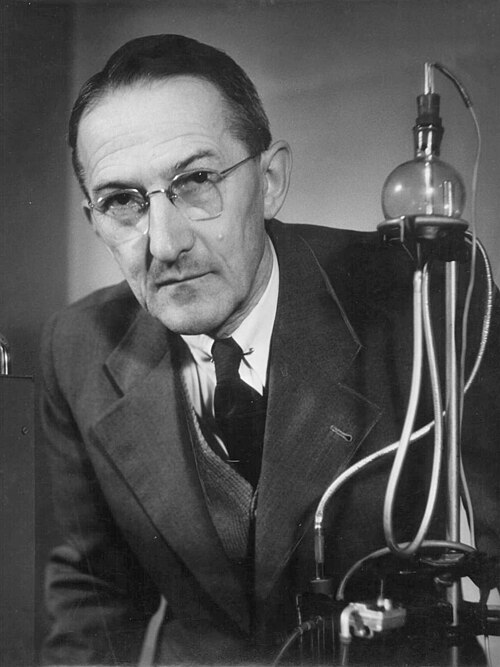
\includegraphics[width=\linewidth]{images/book3/heyrovsky.jpg}
\end{minipage}\hfill
\begin{minipage}[t]{0.71\linewidth}
\vspace{0pt}
Pada tahun 1922 Jaroslav Heyrovský merekam arus yang melewati elektrode
raksa yang terbentuk tetes demi tetes di ujung kapiler, sementara
potensialnya disapu: setiap spesies yang dapat direduksi memberikan sebuah
anak tangga yang posisinya mengidentifikasinya dan tingginya mengukur
konsentrasinya. Tetes yang terus diperbarui menjaga permukaannya tetap
segar, dan \omterm{def:b2:current-potential-curves:overpotential}{overpotensial} hidrogen yang tinggi pada raksa membuka jendela
katodik yang lebar. Polarografi membawanya meraih Hadiah Nobel Kimia pada
tahun 1959 dan melahirkan kimia elektroanalitik; foto ini menunjukkan
dirinya dengan elektrode tetes raksa. (Foto: arsip Institut Kimia Fisika
J.~Heyrovský, CC BY-SA 3.0, Wikimedia Commons.)
\end{minipage}
\end{history}

\section{Latihan}

\begin{exercise}[$\star$]\label{exo:b2:current-potential-curves:1}
Dalam sel Daniell yang memberikan arus, berikan tanda arus pada elektrode
seng dan pada elektrode tembaga, dengan konvensi bab ini.
\end{exercise}

\begin{exercise}[$\star$]\label{exo:b2:current-potential-curves:2}
Hitunglah \omterm{def:b2:current-potential-curves:limiting-current}{arus pembatas} reduksi \ce{Ag+} (\qty{2.0}{mmol/L},
$D =
\qty{1.6e-9}{m^2/s}$) pada \qty{0.50}{cm^2} dengan
$\delta = \qty{25}{\micro m}$ (nilai-nilai model).
\end{exercise}

\begin{exercise}[$\star$]\label{exo:b2:current-potential-curves:3}
Pada kurva-kurva model dalam bab ini, bagaimana mengenali \omterm{def:b2:current-potential-curves:fast-slow}{sistem cepat} dan
\omterm{def:b2:current-potential-curves:fast-slow}{sistem lambat}? Berikan satu contoh masing-masing pada platina.
\end{exercise}

\begin{exercise}[$\star$]\label{exo:b2:current-potential-curves:4}
Sebuah larutan hanya mengandung \ce{Fe^2+}. Pada potensial berapa \omterm{def:b2:current-potential-curves:ie-curve}{arus
anodiknya} mencapai setengah platonya, jika kedua bentuk berdifusi dengan
cara yang sama ($E^\circ = \qty{0.77}{V}$)?
\end{exercise}

\begin{exercise}[$\star\star$]\label{exo:b2:current-potential-curves:5}
Elektrode platina dalam larutan \ce{Fe^3+} dan \ce{Cu^2+} (konsentrasi
sama, $E^\circ$ = 0.77 dan \qty{0.34}{V}) disapu ke arah potensial negatif.
Uraikan kurvanya: gelombang, plato, tingginya, dan dinding katodiknya.
\end{exercise}

\begin{exercise}[$\star\star$]\label{exo:b2:current-potential-curves:6}
Dalam larutan pada \cref{exo:b2:current-potential-curves:5}, potensial
elektrode dijaga pada \qty{0.50}{V}, lalu pada \qty{0.10}{V}. Apa yang
terjadi dalam setiap kasus?
\end{exercise}

\begin{exercise}[$\star\star$]\label{exo:b2:current-potential-curves:7}
Berikan potensial Nernst kedua pasangan air pada pH 0 dan pH 14, lalu
buatlah sketsa bagaimana jendela pada platina bergeser terhadap pH.
\end{exercise}

\begin{exercise}[$\star\star$]\label{exo:b2:current-potential-curves:8}
\ce{Fe^2+} dititrasi dengan \ce{Ce^4+} sementara elektrode platina yang
dijaga pada \qty{1.0}{V} merekam arus. Sketsalah arus terhadap volume yang
ditambahkan, lalu jelaskan bagaimana arus itu menunjukkan letak ekuivalensi
(\ce{Ce^4+}/\ce{Ce^3+}: $E^\circ =
\qty{1.72}{V}$).
\end{exercise}

\begin{exercise}[$\star\star$]\label{exo:b2:current-potential-curves:9}
Menggandakan kecepatan pengadukan membagi dua tebal \omterm{def:b2:current-potential-curves:limiting-current}{lapisan difusi}. Apa
yang terjadi pada plato, potensial setengah gelombang, dan potensial arus
nol sebuah \omterm{def:b2:current-potential-curves:fast-slow}{sistem cepat}?
\end{exercise}

\begin{exercise}[$\star\star\star$]\label{exo:b2:current-potential-curves:10}
Turunkan persamaan gelombang \omterm{def:b2:current-potential-curves:fast-slow}{sistem cepat} dengan hanya bentuk tereduksi
(Red) yang ada, lalu
tunjukkan bahwa alur $E$ terhadap $\log[i/(i_{\lim} - i)]$ merupakan garis
lurus dengan kemiringan $0.059/n$ volt pada \qty{25}{\degreeCelsius}.
\end{exercise}

\begin{exercise}[$\star\star\star$]\label{exo:b2:current-potential-curves:11}
Sepotong seng yang dicelupkan ke dalam asam \qty{1}{mol/L} hanya larut
perlahan, sedangkan potongan yang sama yang menyentuh kawat platina larut
dengan cepat, dengan gelembung hidrogen pada platina. Jelaskan dengan
\omterm{def:b2:current-potential-curves:ie-curve}{kurva arus--potensial}.
\end{exercise}

\begin{exercise}[$\star\star\star$]\label{exo:b2:current-potential-curves:12}
Untuk mengoksidasi spesies yang gelombangnya terletak pada \qty{2.0}{V}
pada pH 0, manakah yang sebaiknya dipilih, elektrode platina atau elektrode
dengan \omterm{def:b2:current-potential-curves:overpotential}{overpotensial} oksigen yang tinggi? Jelaskan, dan nyatakan apa yang
akan terbentuk jika tidak demikian.
\end{exercise}

\section{Soal: Probe Oksigen untuk Sungai}

\begin{problem}[{Soal akhir pekan --- katode sensor oksigen amperometrik,
arus pembatas melalui membrannya, kalibrasi dalam air yang jenuh udara
dengan hukum Henry, dan kadar oksigen sebuah sungai}]
\label{pb:b2:current-potential-curves:1}
Sebuah probe oksigen amperometrik mempunyai katode emas dan anode perak
dalam gel kalium klorida, yang dipisahkan dari sampel oleh membran tipis
yang permeabel terhadap gas. Katode dijaga pada \qty{-0.60}{V} terhadap
anode perak--perak klorida. Data pada \qty{25}{\degreeCelsius}: tetapan
\omterm{prop:b2:chemical-potential:henry}{hukum Henry} untuk \ce{O2}, $H = \qty{1.3e-5}{mol/(m^3.Pa)}$; tekanan uap
air \qty{3.17}{kPa}; oksigen dalam udara kering 20.95~\% volume;
$E^\circ(\ce{O2}/\ce{H2O}) =
\qty{1.229}{V}$;
$E^\circ(\ce{AgCl}/\ce{Ag}) = \qty{0.222}{V}$. Membran (nilai-nilai model):
luas \qty{0.10}{cm^2}, tebal \qty{25}{\micro m}, koefisien difusi efektif
\ce{O2} melintasinya \qty{1.0e-10}{m^2/s}.
% ledger: henry:O2, pvap:H2O.298, air:O2, dfg:Cl-_ao, dfg:AgCl_cr, aw:O

\medskip
\noindent\textbf{Bagian I --- Katode.}
\begin{enumerate}
  \item Tuliskan reduksi dioksigen dalam medium netral.
  \item Tuliskan reaksi di anode perak, serta reaksi keseluruhannya.
  \item Hitunglah potensial Nernst pasangan \ce{O2}/\ce{H2O} pada pH 7 dengan
        $p_{\ce{O2}} = \qty{0.21}{bar}$.
  \item Nyatakan potensial katode, \qty{-0.60}{V} terhadap Ag/AgCl, pada
        skala hidrogen, dengan menganggap aktivitas klorida dalam gel sama
        dengan 1.
  \item Mengapa katode harus dijaga jauh di bawah potensial Nernst \ce{O2}?
  \item Mengapa dipilih potensial yang terletak pada plato?
  \item Apa yang menetapkan batas bawah potensial yang dapat dipakai?
\end{enumerate}

\medskip
\noindent\textbf{Bagian II --- \omterm{def:b2:current-potential-curves:limiting-current}{Arus pembatas}.}
\begin{enumerate}[resume]
  \item Uraikan profil konsentrasi \ce{O2} melintasi membran ketika katode
        bekerja pada platonya.
  \item Tuliskan fluks \ce{O2} melalui membran.
  \item Simpulkan arus sebagai fungsi konsentrasi $c$ \ce{O2} terlarut.
  \item Mengapa tebal membran dipakai sebagai pengganti \omterm{def:b2:current-potential-curves:limiting-current}{lapisan difusi}?
  \item Mengapa pembacaannya hanya sedikit bergantung pada pengadukan air
        sungai, tetapi sangat bergantung pada kotornya membran?
\end{enumerate}

\medskip
\noindent\textbf{Bagian III --- Kalibrasi.}
\begin{enumerate}[resume]
  \item Hitunglah tekanan parsial \ce{O2} di atas air yang jenuh udara pada
        \qty{1.013}{bar} dan \qty{25}{\degreeCelsius}.
  \item Hitunglah konsentrasi \ce{O2} terlarut pada keadaan jenuh, dalam
        \unit{mol/m^3}.
  \item Nyatakan nilai itu dalam \unit{mg/L}.
  \item Ramalkan arus probe dalam air yang jenuh udara.
  \item Probe itu sebenarnya membaca \qty{4.05}{\micro A} dalam air yang
        jenuh udara (data latihan). Hitunglah kepekaannya dalam
        \unit{\micro A} per \unit{mg/L}.
  \item Mengapa probe dikalibrasi alih-alih memercayai arus yang
        diramalkan?
  \item Apa yang seharusnya dibaca probe dalam air yang dibebaskan dari
        oksigen?
\end{enumerate}

\medskip
\noindent\textbf{Bagian IV --- Sungai.}
\begin{enumerate}[resume]
  \item Dalam sampel air sungai pada \qty{25}{\degreeCelsius}, probe
        membaca \qty{2.80}{\micro A}. Hitunglah oksigen terlarutnya dalam
        \unit{mg/L}.
  \item Nyatakan nilai itu sebagai persentase kejenuhan.
  \item Air sebuah sungai hampir jenuh oksigen di sumbernya. Usulkan
        penyebab kekurangannya.
  \item Berapa jumlah \ce{O2} yang dikonsumsi probe dalam satu jam? Apakah
        probe itu mengganggu sampel?
  \item Mengapa kalibrasi harus diulang jika sungainya bersuhu
        \qty{15}{\degreeCelsius}?
  \item Nyatakan konsentrasi oksigen terlarut dalam sampel itu.
\end{enumerate}
\end{problem}
